\section{Experiments}\label{sec:main_experiments}

\subsection{Experimental setup}

% \paragr{Platform.}
\textbf{VirtualHome.}
We proceed with our experiments in the VirtualHome \cite{puig2018virtualhome}, a large household simulated environment with a large domain, partial observations, and large action space. It contains hundreds of interactive items and containers with various types of rooms. It is a well-suited platform for evaluating embodied decision-making for solving daily tasks in household environments.
% Same as prior works \cite{li2022pre}, to enable using LLM, we transform the agent's partial observations and goals in VirtualHome into English sentences. 
% We use object names and their relations to containers, surfaces, and rooms as the observation.

% Similar to \cite{li2022pre}, the VirtualHome environment is structured within a POMDP model. A state is represented by a set of variables representing the position of each object and robot in a house, where the value of a position is the spatial relations to another object. The robot can pick a grabbable object if the object is nearby and not inside a closed container. It can place a grabbable object in a place if the placement is nearby and not the space inside a closed container. It can also move to a connected room and open or close a nearby container. Observations are a subset of the objects and their positions because the robot's perception is limited to unobstructed objects within its immediate vicinity. The reward identifies the goal of the task and is positive if the goal is achieved and zero otherwise. 

% This model employs an object-centric graph to define states, where nodes represent objects characterized by attributes such as type and position, while edges illustrate inter-object relationships. Belief states manifest as distributions over this graph, with each node fully interconnected and edges attached with probabilistic values, indicating relationship likelihoods. Given a state, action transitions are deterministic and modify the state graph's connectivity. For instance, when an apple is on a table, an ``on'' edge exists between the ``apple'' and ``table'' nodes. Picking up the apple removes this edge, introducing a new ``hold'' connection between the ``apple'' and ``robot'' nodes. Observations are subgraphs of the state graph because the robot's perception is limited to unobstructed objects within its immediate vicinity. The reward identifies the goal of the task and is positive if the goal is achieved and zero otherwise. 


% \textbf{Task.} 


\textbf{Data.}
To generate data for prompting and baseline training, we follow \cite{puig2020watch} to create 2000 tasks with randomly initialized scenes and expert trajectories. There are several settings for the evaluation. \textit{Simple} tasks are the tasks that only require the rearrangement of one item generated from the same distribution as the training dataset. \textit{Comp.} refers to the composition of simple tasks in order to rearrange multiple objects sampled from the same distribution as the dataset (e.g., ``Put plate on kitchen table and chicken inside fridge'' is the composition of ``put plate on kitchen table'' and ``put chicken inside fridge,'' ). The composition of tasks increases the planning horizon, making it more challenging to complete.
In evaluation, we also use the \textit{Novel Simple} tasks with seen items 
(e.g., in the dataset, we have ``put one plate on the kitchen table'' and ``put one chicken inside the fridge,'' and we use ``put one plate inside the fridge'' and ``put one chicken on the kitchen table'' to evaluate; these tasks are not included in the training dataset). 
For compositional tasks, we include \textit{Novel Comp}ositional tasks, with 2 or 3 primary tasks composed, denoted as \emph{NovelComp(2)} and \emph{NovelComp(3)} (e.g., we have ``put plate on kitchen table'' and ``put chicken inside fridge,'' in dataset but their composition ``Put plate on kitchen table and chicken inside fridge'' is not.) We also generate scenes at a \textit{Novel Apartment} for testing, where the distribution of object positions differs from the dataset. 

The expert data are generated by an Oracle agent implemented in~\cite{puig2020watch}. The expert has the full knowledge of the environment (hence, does not need to understand where objects are likely to be placed) and uses handcrafted heuristics for completing various tasks. It uses regression planning to search for solutions to a task. We collect the actions and observations of the expert completing the tasks in the VirtualHome simulator as the dataset. There are 10,000 trajectories in total for training the baseline. To show the capability of LLMs when using a small training set, we only select 200 instances uniformly at random from the dataset as prompt candidates for the LLM model and policy when used in a few-shot mode with no fine-tuning. We also generated 800 tasks in total for evaluation. 

\textbf{Evaluation.} We evaluate the success rate of completing the tasks within 30 steps, while a typical task can be finished within at most 15 steps. The task is considered successful if all the requirements of object positions are satisfied. For example, given the instruction ``Put one apple inside the fridge,'' the task is successful if any apple is in the fridge. For simplicity, we don't consider the task of rearranging a very specific object, e.g., putting the leftmost apple in the fridge. 

\textbf{Baselines.} 
We evaluate several baselines to compare. \textit{UCT}~\cite{kocsis2006bandit}: We use the UCT algorithm to conduct planning without commonsense knowledge and use the ground-truth reward function in simulation. We use uniform distribution as the initial belief for states of objects. It is to provide evidence that commonsense knowledge improves planning efficiency.
\textit{Finetuned GPT2 policy} \cite{li2022pre}: we use the training dataset with 10000 trajectories to fine-tune GPT-2 as the planning policy. This is to show that larger pre-trained LLM without fine-tuning outperforms the smaller model fine-tuned in specific tasks. 
\textit{GPT3.5 Policy} \cite{huang2022language}: 
LLM takes as input the instructions and history of actions and the currently visible objects to generate the next action. 
We use the LLM as the policy only, with a few examples as prompts to interact with the environments. 
% \begin{table}[t]
\begin{wraptable}[10]{r}{0.68\columnwidth}
\vspace{-15pt}
\setlength\extrarowheight{-3pt}
\setlength\tabcolsep{2pt}
\centering\scriptsize
\caption{Main results: mean $\pm$ standard error of success rate (\%)}
\begin{tabular}{@{}cccccc@{}}
\toprule
                  & \multicolumn{5}{c}{Seen}                          \\ \cmidrule(l){2-6} 
Method            &  Simple &  Comp. & NovelSimple & NovelComp.(2) & NovelComp.(3) \\ \midrule
UCT \cite{kocsis2006bandit} &  0.0$\pm$0.0        &  0.0$\pm$0.0       &  0.0$\pm$0.0       & 0.0$\pm$0.0    & 0.0$\pm$0.0  \\
finetuned GPT2 policy~\cite{li2022pre}  &   81.3$\pm$2.4    &  59.0$\pm$6.7        &  41.2$\pm$7.1      &    30.9$\pm$2.8     &  2.3$\pm$1.5           \\
GPT3.5 Policy~\cite{huang2022language} &   83.4$\pm$6.8  &  47.0$\pm$7.8      &    74.3$\pm$4.0      &     48.2$\pm$8.8      &    5.4$\pm$2.0     \\
GPT3.5-MCTS (Ours)      & 91.4$\pm$3.3   &  71.2$\pm$6.2    &  88.1$\pm$4.3   &  72.6$\pm$6.9       &      33.6$\pm$3.1        \\ \toprule
                  & \multicolumn{5}{c}{Unseen}                   \\ \cmidrule(l){2-6} 
Method            &  Simple &  Comp.  & NovelSimple & NovelComp.(2) & NovelComp.(3) \\ \midrule
UCT \cite{kocsis2006bandit} &   0.0$\pm$0.0      &  0.0$\pm$0.0        &  0.0$\pm$0.0         &    0.0$\pm$0.0           &    0.0$\pm$0.0   \\
finetuned GPT2 policy~\cite{li2022pre} &    65.5$\pm$3.4     &  39.9$\pm$5.2      &  33.4$\pm$6.4         &  12.8$\pm$3.9           &    1.1$\pm$0.9    \\
GPT3.5 Policy~\cite{huang2022language} &   74.3$\pm$5.0     &  43.3$\pm$4.0       &  67.8$\pm$4.9        &     54.0$\pm$3.0       &   6.9$\pm$2.1  \\
GPT3.5-MCTS (Ours)    &  82.9$\pm$3.2   &  71.9$\pm$5.6    &  79.3$\pm$3.3   &   70.4$\pm$6.4      &   38.8$\pm$3.4  \\ \bottomrule
\end{tabular}
\label{tab:main}
% \end{table}
\end{wraptable}
This baseline demonstrates the benefits of additional information from the commonsense model and algorithmic benefits from MCTS. 


% For implementation, we use GPT-3.5 as the LLM. The temperature parameter is set to 0.6, and the top-p parameter is 0.9. The sample number for querying the LLM is $M=10$, and the number of prompts is $K=1$. The mixture parameter for heuristic policy is $\lambda=0.5$. We select 200 instances uniformly at random from the dataset as prompt candidates for the LLM model and policy. Other details are enclosed in the appendix of the supplementary materials. 

\subsection{Results}

\textbf{Main result.}
The main results of the experiments are shown in Table \ref{tab:main}, reporting the success rate of our method and baselines in completing the tasks in VirtualHome environments. In this result, GPT3.5-MCTS outperforms all the compared baselines, especially for unseen situations. UCT works poorly in all conditions, as the poor model and the huge search tree make the planning intractable. Thus, we focus our discussion on comparing the finetuned GPT2 policy and GPT3.5 policy. 
For \textit{Simple}, in-distribution tasks, the planning horizon is relatively short. Finetuned GPT2 policy, GPT3.5 Policy, and our method work reasonably well, but our method still outperforms the baselines. For \textit{Novel Simple} tasks, finetuned GPT2 policy works significantly worse than GPT3.5 Policy and GPT3.5-MCTS. This is because the fine-tuning of narrow tasks results in a biased distribution of the policy and compromises generalizability. GPT3.5 Policy and GPT3.5-MCTS work better due to the LLM's few-shot planning capability. GPT3.5-MCTS works better for both situations. It benefits from the MCTS' look-ahead search that explore possible states for potential outcomes in order to make reasoned decisions. 
% This procedure utilizes the additional commonsense knowledge of the world encoded in LLM, compared to using LLM solely as policy. 


For the \textit{Comp}ositional, in-distribution tasks, the finetuned GPT2 policy and GPT3.5 policy get significantly worse performance, while GPT3.5-MCTS works far better. The finetuned GPT2 policy is trained by behavior cloning that suffers from compounding errors. Therefore, when the planning horizon gets longer, the influence of the errors accumulates and compromises the overall performance significantly. As for GPT3.5 Policy, the longer horizon potentially introduces more errors during planning, which might not be included in the prompt examples. Without suitable guidance from prompt, we cannot guarantee the GPT3.5 Policy will carry out suitable replanning when encountering errors. MCTS encourages exploration to a certain extent of different possible actions during searching, introducing additional guidance to the GPT3.5 policy to look into other possible solutions. This is because the action selection procedure in GPT3.5-MCTS is not purely determined by GPT3.5 Policy but also by the $Q$ value and visit counts. Thus, MCTS encourages GPT3.5 Policy to explore other possible search directions instead of excessively applying certain actions sampled by itself.  




% \begin{wraptable}[14]{r}{0.6\columnwidth}
% % \begin{table}[h]
% \vspace{-8pt}
% \setlength\tabcolsep{2pt}
% \centering\scriptsize
% \caption{Results on Ablation Study: Success Rate (\%)}
% % \vspace{4pt}
% \begin{tabular}{@{}ccccc@{}}
% \toprule
%                   & \multicolumn{4}{c}{Seen Apartment}                          \\ \cmidrule(l){2-5} 
% Method            &  Simple &  Comp. & NovelSimple & NovelComp. \\ \midrule
% GPT3.5-MCTS (No Heuristic Policy)  &  0.0$\pm$0.0   &   0.0$\pm$0.0       &  0.0$\pm$0.0    &    0.0$\pm$0.0               \\
% GPT3.5-MCTS (Uniform State Prior)  &   3.2$\pm$1.1     &  0.0$\pm$0.0     &  1.1$\pm$0.4       &     0.0$\pm$0.0             \\
% GPT3.5-MCTS (Fully Observable) &   94.0$\pm$2.1    &   80.7$\pm$3.3     &  94.3$\pm$2.4       &     78.5$\pm$4.0               \\
% GPT3.5-MCTS (Ours)      & 91.4$\pm$3.3   &  71.2$\pm$6.2    &  88.1$\pm$4.3   &  72.6$\pm$6.9           
% % GPT3.5-MCTS           &   94.3     &  73.6       &  87.0       &   69.7                    
% \\ \toprule
%                   & \multicolumn{4}{c}{Unseen Apartment}                   \\ \cmidrule(l){2-5} 
% Method            &  Simple &  Comp.  & NovelSimple & NovelComp. \\ \midrule
% GPT3.5-MCTS (No Heuristic Policy)  &  0.0$\pm$0.0    &   0.0$\pm$0.0       &  0.0$\pm$0.0     &    0.0$\pm$0.0                 \\
% GPT3.5-MCTS (Uniform State Prior) &   1.1$\pm$0.2     &  0.0$\pm$0.0      &  0.0$\pm$0.0       &     0.0$\pm$0.0              \\
% GPT3.5-MCTS (Fully Observable) &   85.1$\pm$5.0     &  73.3$\pm$4.2      &  80.1$\pm$3.7       &     71.1$\pm$2.2               \\
% GPT3.5-MCTS (Ours)    &  82.9$\pm$3.2   &  71.9$\pm$5.6    &  79.3$\pm$3.3   &   70.4$\pm$6.4       
% % GPT3.5-MCTS     &   81.3     &  70.4       &  77.5        &    70.0                
% \\ \bottomrule
% \end{tabular}
% \label{tab:ablation}
% % \end{table}
% \end{wraptable}

\textbf{Ablation study.}
We conduct ablation studies to see the individual contributions of different components within the GPT3.5-MCTS framework. The \textit{No Heuristic Policy} version of GPT3.5-MCTS refers to the absence of PUCT guided by the GPT3.5 Policy for action selection. Instead, it solely relies on UCT with an initial commonsense belief derived from LLM. The variant employing the \textit{Uniform State Prior} utilizes a uniform prior belief regarding states, in contrast to the LLM-generated initial belief employed during the search process. Lastly, the variant operating in a \textit{Fully Observable} environment aims to assess the accuracy of LLM's knowledge in modeling the world.

\begin{table}[h]
\vspace{-5pt}
\setlength\extrarowheight{-3pt}
\setlength\tabcolsep{2pt}
\centering\scriptsize
\caption{Results on Ablation Study:  mean $\pm$ standard error of success rate (\%)}
\vspace{-7pt}
\begin{tabular}{@{}ccccccccc@{}}
\toprule
                  & \multicolumn{4}{c}{Seen Apartment}       & \multicolumn{4}{c}{Unseen Apartment}                      \\ \cmidrule(l){2-5} \cmidrule(l){6-9}
Method            &  Simple &  Comp. & NovelSimple & NovelComp.(2)  &  Simple &  Comp. & NovelSimple & NovelComp.(2)\\ \midrule
GPT3.5-MCTS (No Heuristic Policy)  &  0.0$\pm$0.0   &   0.0$\pm$0.0       &  0.0$\pm$0.0    &    0.0$\pm$0.0    &  0.0$\pm$0.0    &   0.0$\pm$0.0       &  0.0$\pm$0.0     &    0.0$\pm$0.0              \\
GPT3.5-MCTS (Uniform State Prior)  &   3.2$\pm$1.1     &  0.0$\pm$0.0     &  1.1$\pm$0.4       &     0.0$\pm$0.0     &   1.1$\pm$0.2     &  0.0$\pm$0.0      &  0.0$\pm$0.0       &     0.0$\pm$0.0             \\
GPT3.5-MCTS (Fully Observable) &   94.0$\pm$2.1    &   80.7$\pm$3.3     &  94.3$\pm$2.4       &     78.5$\pm$4.0       &   85.1$\pm$5.0     &  77.5$\pm$3.2      &  82.2$\pm$3.3       &     76.6$\pm$3.1            \\
GPT3.5-MCTS (Ours)      & 91.4$\pm$3.3   &  71.2$\pm$6.2    &  88.1$\pm$4.3   &  72.6$\pm$6.9    &  82.9$\pm$3.2   &  71.9$\pm$5.6    &  79.3$\pm$3.3   &   70.4$\pm$6.4        
% GPT3.5-MCTS           &   94.3     &  73.6       &  87.0       &   69.7                    
% \\ \toprule
%                   & \multicolumn{4}{c}{Unseen Apartment}                   \\ \cmidrule(l){2-5} 
% Method            &  Simple &  Comp.  & NovelSimple & NovelComp. \\ \midrule
% GPT3.5-MCTS (No Heuristic Policy)  &  0.0$\pm$0.0    &   0.0$\pm$0.0       &  0.0$\pm$0.0     &    0.0$\pm$0.0                 \\
% GPT3.5-MCTS (Uniform State Prior) &   1.1$\pm$0.2     &  0.0$\pm$0.0      &  0.0$\pm$0.0       &     0.0$\pm$0.0              \\
% GPT3.5-MCTS (Fully Observable) &   85.1$\pm$5.0     &  73.3$\pm$4.2      &  80.1$\pm$3.7       &     71.1$\pm$2.2               \\
% GPT3.5-MCTS (Ours)    &  82.9$\pm$3.2   &  71.9$\pm$5.6    &  79.3$\pm$3.3   &   70.4$\pm$6.4       
% % GPT3.5-MCTS     &   81.3     &  70.4       &  77.5        &    70.0                
\\ \bottomrule
\end{tabular}
\label{tab:ablation}
\vspace{-8pt}
\end{table}

Table \ref{tab:ablation} presents the results of our ablation experiments. The outcomes obtained under the \textit{No Heuristic Policy} version highlight the significance of heuristic policies in facilitating MCTS to conduct efficient searches for complex and large-scale planning tasks. Conversely, the results of the \textit{Uniform State Prior} row indicate that incorrect world models compromise search performance. This is because the model of the world determines the $Q$ value. The wrong model results in an inaccurate estimation of the $Q$ value, misleading the search process toward irrelevant locations. The \textit{Fully Observable} results demonstrate that GPT3.5-MCTS with perfect knowledge of the environment only slightly outperforms its counterpart without it, implying that the commonsense knowledge of LLM regarding world modelling suffices for practical purposes.



% \begin{table}[h]
% \centering\scriptsize
% \caption{Results on Ablation Study: Success Rate (\%)}
% \begin{tabular}{@{}ccccc@{}}
% \toprule
%                   & \multicolumn{4}{c}{Seen Apartment}                          \\ \cmidrule(l){2-5} 
% Method            &  Simple &  Comp. & Novel Simple & Novel Comp. \\ \midrule
% GPT3.5-MCTS (No Heuristic Policy)  &  0.0    &   0.0       &  0.0     &    0.0                 \\
% GPT3.5-MCTS (Uniform State Prior)  &   0.0     &  --      &  0.0       &     --             \\
% GPT3.5-MCTS (Fully Observable) &   97.0     &   80.7     &  94.3       &     78.5               \\
% GPT3.5-MCTS           &   94.3     &  73.6       &  87.0       &   69.7                    \\ \toprule
%                   & \multicolumn{4}{c}{Unseen Apartment}                   \\ \cmidrule(l){2-5} 
% Method            &  Simple &  Comp.  & Novel Simple & Novel Comp. \\ \midrule
% GPT3.5-MCTS (No Heuristic Policy)  &  0.0    &   0.0       &  0.0     &    0.0                 \\
% GPT3.5-MCTS (Uniform State Prior) &   0.0     &  --      &  0.0       &     --               \\
% GPT3.5-MCTS (Fully Observable) &   85.1     &  --      &  80.1       &     --               \\
% GPT3.5-MCTS     &   81.3     &  70.4       &  77.5        &    70.0                 \\ \bottomrule
% \end{tabular}
% \label{tab:ablation}
% \end{table}

\textbf{Failure analysis.}
Policy, model, and translation errors are the primary causes of failures. Among these, policy errors are responsible for the majority of the failures. Oftentimes, the policy produces unreasonable behaviours that mislead the search procedure. For example, it usually outputs inadmissible actions, such as ``\textit{walk to the cutleryfork}'' where the ``\textit{cutleryfork}'' is not in the observation. It also produces back-and-forth behaviours, resulting in an unreasonable heuristic and slowing the search procedure. For example, when putting objects inside the microwave, it is sometimes struck by repeatedly opening and closing the microwave. For model error, the predicted positions of objects are not always correct. Since a random rollout policy is employed, incorrect object states can result in higher $Q$-values than correct states, leading to misguided exploration. The wrong translation also compromises the performance as we translate the response from LLM to admissible action or object names to ensure executability. This is partly caused by the VirtualHome environments, as the policy might not understand the underlying logic of the actions in VirtualHome, such as you have to walk close to interact with the object. Thus, if the LLM outputs ``open fridge'' but is not close enough to the fridge, the action will be translated to other admissible actions (``open fridge'' is not inside the admissible actions for this case as it is invalid due to the setting of VirtualHome). 

\section{LLM as a model or a policy?}\label{sec:mdl}

{
% \color{blue}

%To explain why using LLM as a model in LLM-MCTS works well, we discovered that for certain real-world domains, if the description length of the world model is shorter than policy, using LLM as a model in model-based planning is likely better than using LLM solely as a policy. The description length can be represented by the minimum complexity of describing the solution of a problem. See Introduction \ref{sec:intro} and section \ref{sec:air-plan} for concrete examples. 

When would using LLM as a model outperform using LLM as a policy, and vice versa? We propose using the minimum description length (MDL) principle, also known as Occam's Razor from the philosophy of science, to gain insights into the issue. The MDL principle suggests choosing the method that has a shorter description when both methods fit the training data well. MDL has been formalized in various ways. One formal statement (from section 7.3 of \cite{shalev2014understanding}) is provided here:
\begin{theorem}[Occam's Razor]
Let $\mathcal{H}$ be a hypothesis class and let $d:\mathcal{H} \rightarrow \{0, 1\}^*$ be a prefix-free description language for $\mathcal{H}$. Then, for every sample size, $m$, every confidence parameter, $\delta > 0$, and every probability distribution, $D$, with probability greater than $1-\delta$ over the choice of $S\sim D^m$ we have that,
$ \forall h\in\mathcal{H}, L_D(h)\leq L_S(h)+\sqrt{(|h|+\ln{(2/\delta)})/2m}
$
where $L_S(h)$ is the empirical loss of $h$ on the $S$, $L_D(h)$ is the expected loss of $h$, and $|h|$ is the length of $d(h)$.
\vspace{-4pt}
%    Let $\mathcal{H}$ be a prediction rule class and let $d:\mathcal{H} \rightarrow \{0, 1\}^*$ be a prefix-free description language for $\mathcal{H}$. {\color{purple}$d(h)$ is the description of $h$, and $|h|$ is the length of $d(h)$, which can be evaluated by the bits of space complexity of $d(h)$}. The error rate is $err_D(h)=\mathbb{P}_{x\in D}[h(x)\neq c(x)]$ where $c(x)$ is the label of $x$. For every sample size $m$, every confidence parameter, $\delta > 0$, and every probability distribution, $D$, with probability greater than $1-\delta$ over the choice of $S\sim D^m$ we have that, $
 %       \forall h\in\mathcal{H}, err_D(h)\leq err_S(h)+\sqrt{(|h|+\ln{(2/\delta)})/2m}.
 %   $
\label{theorem:or_main}
\end{theorem}
According to Theorem \ref{theorem:or_main}, we can bound the expected loss of a solution $h$ by the description length $|h|$ and the training loss $L_S(h)$. We do not know the LLM training loss for using it as a model or as a policy, but for the purpose of gaining insights, it is reasonable to assume that they are both small. In that case, the MDL principle suggests selecting between a model or policy depending on which of them has the smaller description length given the description language.

Numerous caveats should be observed when using Theorem \ref{theorem:or_main} to gain insights into the behaviour of LLM as a model and policy. The theorem assumes that the training data is independent and identically distributed (iid), which is likely not true in practice. Nonetheless, the qualitative behaviour is often similar for non-iid data. 
% Second, the theorem only provides an upper bound on the error; again, with care, comparing upper bounds may provide some insights. 
%Second, the result depends on the description language used; we assume that comparison is reasonable under a reasonable choice of description languages. 
In addition, using the theorem to gain insights requires major assumptions on the predictor classes $\mathcal{H}$ for model and policy; here, we assume that $\mathcal{H}$ is the model (or policy) class that we are analysing and assume that LLM training using powerful approximators such as transformers has similar behaviour to training using the model (or policy) class. Finally, depending on how the model and policy are used, error propagation may need to be analysed separately. 

Besides the multiplication example described earlier, we discuss an air travel planning task and the VirtualHome object rearrangement task examined earlier.

% In the learning procedure, $h$ minimizes the empirical error (ideally, the learning algorithm aims to achieve $err_S(h)\rightarrow 0$). Thus, with a fixed size of data $m$, if the description length for model prediction is smaller than policy prediction, LLM would make fewer mistakes when building the world model than being used as a policy directly. 
% We use the object rearrangement results to analyze this finding and further verify this finding by an additional air travel planning experiment and analysis. 

% When training data is \textbf{not} unlimited, LLM's knowledge about the world model is likely more complete than the policy in many domains, as learning policy is more data-consuming than learning the world model. We analyze the sample efficiency using the description lengths of both the world model and the policy. The description length, reflecting the space complexity to represent full knowledge, determines the data needed to cover situations in a task or domain. 

\iffalse
Then, we analyze how the error is propagated when solving multi-step planning problems. Consider a planning problem that combines $k$ elementary tasks from a task space $\Omega$, and solving each elementary task requires $\phi$ steps on average. Thus, the size of the solution space is $O(|\Omega|^{k}\phi)$ as we need to consider arbitrary combinations of $k$ elementary tasks. Describing a policy with full solutions requires $O(|\Omega|^k\phi)$ bits. As shown in Theorem \ref{theorem:or_main}, it makes the error rate bound to blow up, indicating the LLM policy could make exponentially more errors. Assume the error rate of LLM in predicting a world model is $\epsilon$ and acting as a policy to solve the above problem is $\zeta(k)$. If the description length of the world model is substantially smaller than the shortest policy $O(|\Omega|\phi)$ (i.e., the policy when $k=1$), then, according to Theorem \ref{theorem:or_main}, there should be $\epsilon \ll \zeta(1) < \zeta(k)$. To do the multi-step planning, the model-based approach accumulates errors made by LLM's world model. Assuming the mistakes made by the LLM models for each step are independent with mostly the same probability, then the accuracy of the model-based approach should be $(1-\epsilon)^{\phi k}$ after $\phi k$ steps of planning if analyzed naively. 
 Thus, we have the following analysis. 
 \begin{proposition}[informal]
Consider a planning problem that combines $k$ elementary tasks from a task space $\Omega$, and solving each elementary task requires $\phi$ steps on average. If the description length of the world model is substantially smaller than the shortest policy $O(|\Omega|\phi)$, there should exist a moderate value for $\hat{k}>0$ and $\hat{\phi}>0$ such that when $\phi k < \hat{\phi} \hat{k}$,
% \begin{equation}
    $(1-\epsilon)^{\phi k}> 1-\zeta(k)$,
% \end{equation}
indicating that for a planning task with $k$ and $\phi$ satisfying the above condition, the LLM model-based method works better than the LLM policy. Otherwise, both methods should work equally well due to the over-simple planning task, or poorly due to the exponentially grown error. 
 \end{proposition}
\fi
 
% Then, we analyze how the error is propagated when solving multi-step planning problems. Assume the error rate of LLM in predicting a world model is $\epsilon$ and acting as a policy is $\zeta$. If the description length of the world model is substantially smaller than the policy, then there should be $\epsilon \ll \zeta$. Generally, planning is a hard combinatorial search problem \cite{kautz1996pushing}, making the description length of the solution grow exponentially \cite{ weld1999recent}. As shown in Theorem \ref{theorem:or_main}, it makes the error rate bound to blow up, indicating the LLM policy could make exponentially more errors. To do the multi-step planning, the model-based approach accumulates errors made by LLM's world model. Assuming solving elementary tasks requires a constant step $\phi$ on average, the mistakes made by the LLM models for each step are independent with mostly the same probability, then the accuracy of the model-based approach should be $(1-\epsilon)^{\phi k}$ after $\phi k$ steps of planning if analyzed naively. 
%  Thus, we have: 
%  \begin{proposition}[informal] 
% If $\forall k, \epsilon \ll \zeta(k)$ and $\zeta(k)$ grows when $k$ increases, there should exist a moderate value for $\hat{k}$ and $\hat{\phi}$ such that $\forall \phi, k$, if $\phi k < \hat{\phi} \hat{k}$, then
% % \begin{equation}
%     $(1-\epsilon)^{\phi k}> 1-\zeta(k)$,
% % \end{equation}
% indicating that for a planning task with $k$ and $\phi$ satisfying the above condition, the LLM model-based method works better than the LLM policy. Otherwise, both methods should work equally well due to the over-simple planning task, or poorly due to the exponentially grown error. \label{pre:ineq}
%  \end{proposition}The detailed proof of Proposition \ref{pre:ineq} is shown in the Appendix. 

}

\subsection{Travel planning}\label{sec:air-plan}

{
% \color{blue}

Consider planning for air travel from a starting city to the destination city. To solve the problem through L-Model, we need to have the model -- the direct flights out of each city -- together with a shortest path algorithm. The model can be represented as a graph, which is likely to be sparse in the real world. 
For a sparse graph, an adjacency list will give a compact representation. 
Assuming that the total number of edges grows proportionally to the number of cities, $O(n\log n)$ bits would be sufficient to describe a graph with $n$ cities, with approximately $\log n$ bits used to describe each city in the adjacency list structure. The shortest path algorithm can be described by any reasonable programming language with a constant size. 
The method regarding L-Policy 
% is to describe the next city to fly to from the current city (including the start city) along the path to the goal. This can be represented 
can be represented as a 2-dimensional table, where each row and column denotes the current and destination city, and the table entry describes the next city to fly to on the shortest path from the current city to the destination. The next city in the table can be described with $\log n$ bits. As such, with $n$ cities in the rows and columns, there should be approximately $n^2\log n$ bits in total. Thus, according to MDL, the L-Model has a shorter description length and should make fewer generalization errors than the L-Policy for travel planning with sufficiently large $n$. 

\textbf{Experiment.} 
We conducted experiments about planning for air travel from a starting city to a destination city, which we analyzed above. We utilized GPT-3.5 to generate flight paths between cities. We compare it to the GPT-3.5 model-based approach: we use GPT-3.5 to predict neighbouring cities connected by a direct flight, which feeds into the uniform-cost search (i.e., replace node expansion by GPT-3.5 as the world model). 

We use the data from the Kaggle World cities database, select 68 cities with populations exceeding 5 million in different countries and 62 middle-size cities with populations between 500 thousand and 2 million, and use the Virtual Radar Server to get the flight routes dataset as ground truth. In our tests, we sampled 400 city pairs among large cities and 400 pairs among mid-size cities, evaluating path accuracy by verifying each direct flight exists. Paths were accepted if all flights were valid, even if they extended beyond our selected source and target cities. 
We evaluate the methods in two settings: predicting the flight route given two large cities and two mid-size cities.

%We use GPT-3.5 in a model-based method, which predicts direct-flight-connected cities integrated into a uniform-cost search. Using the Kaggle World Cities database, we chose 68 large cities (population > 5 million) to assess in our main experiments. Flight route validation came from the Virtual Radar Server. We evaluated 400 pairs from each city category, verifying the existence of direct flights. Valid paths contained only legitimate flights, even if they exceeded the chosen cities. Our assessment spanned single- and multi-destination routes. The multi-destination route planning from an origin to two to four large cities assesses model compositional generalizability.


\begin{wrapfigure}[8]{r}{0.38\columnwidth}
    \centering
    \vspace{-15pt}
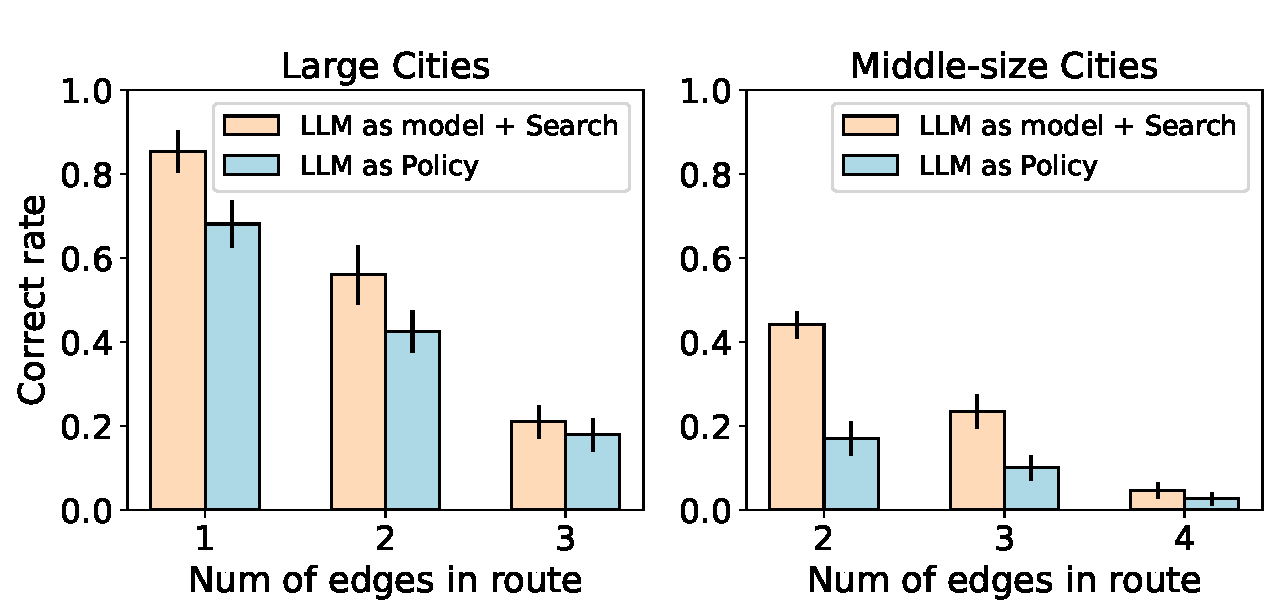
\includegraphics[width=0.38\columnwidth]{img/plot_main_2.pdf}
    \vspace{-15pt}
    \caption{Flight planning results.}
    \label{fig:air-plan-result}
\end{wrapfigure} 
\textbf{Results. }The main result shown in Fig \ref{fig:air-plan-result} suggests that the LLM model + search algorithm consistently outperforms the LLM policy, supporting our analysis\footnote{Single-edge results are omitted for mid-size cities as there are no such routes in the experiments.}. Furthermore, the performance gaps for mid-size cities are larger than for large cities. This is consistent with the fact that there are more mid-size cities than large cities (the gap between the description lengths of $n^2\log n$ for policies vs $n\log n$ for models grows with the number of cities). Note that performance decreases as the path length increases for both methods. As the number of predictions required for each path increases with path length, the probability of incorrect path prediction also increases.
%On the other hand, when the problem becomes more complex, both the model-based and model-free methods become insufficient. The model-based method suffers from the compounding error of imperfect model prediction. Similarly, the LLM policy's error rate grows rapidly due to the increased description length. Detailed results are in the Appendix. 

% \textbf{Monty Hall problem. }
% In addition, there is also a case where the description length of the policy is shorter than the model, and using LLM as a model might be worse than using LLM as a policy. One example could be the Monty Hall problem. In this problem, contestants pick one of three doors: one hides a car, two hide goats, and they will win if they pick the one with a car. The contestant can stick or switch after a goat is revealed behind another door. While a detailed model proves switching has a 2/3 win chance compared to 1/3 for sticking, the policy is succinct: "Always switch doors." Explaining the strategy is complex, but following it is simple, making a direct policy approach more efficient than modeling.

}

\subsection{Object rearrangement task}

Consider a house with $n$ movable objects, $m$ containers, and $k$ rooms. If we use L-Model, we must describe the model and search algorithm (i.e., MCTS). The model can be represented as a sparse graph with objects, containers, and rooms as nodes, and weighted directed edges signifying a "located in" relation between the nodes, with the weights specifying the probabilities. Assume that each weight is specified with a constant number of bits. Each of the $n$ objects can be located within the $m+k$ containers or rooms, so each object edge would require approximately $\log(m+k)$ bits to describe. Each of the $m$ containers can be located in $k$ rooms, so each container edge would require approximately $\log(k)$ bits to describe. Assume further that the degree of each object and container node in the graph is bounded by a constant; the entire graph then requires $O(n\log(m+k)+m\log(k))=O((m+n)\log(m+k))$ bits to describe. The MCTS algorithm should be described by a programming language with a constant size. 
For the L-Policy, tasks can be designated using object-container pairs. Each object-container policy can be defined by a sequence of actions, e.g. ``walk to the fridge, open the fridge,'' until the object is found, followed by a sequence of actions until the destination container is found. Each action takes $O(m+k)$ bits to describe. Assuming search sequences and the size of each object-container policy are bounded by a constant. Describing the policies for all $mn$ object-container pairs requires $O(mn\log(m+k))$ bits. 
% Interestingly, in this case, the policy can be decomposed into a policy for finding the object and a policy for finding the target container, and each policy can be described separately. The description length of the decomposed policy is closer to that of the model. However, the extent to which LLM's learning can approximate learning of the decomposed policy instead of the policy with a higher description length is unclear, with experiments favouring the model-based approach.

% When tasks are compounded, policy description complexity amplifies to $O((mn)^N\log (m+n+k))$, where $N$ represents the count of compounded tasks. The goal identification facet in the model-based approach correspondingly escalates in intricacy. Still, these compound tasks can be segregated into singular tasks executed consecutively. The capacity of LLMs to deconstruct these challenges remains nebulous, though our trials suggest a superior performance for the model-based strategy. Such decomposition is pivotal in diminishing descriptive complexity, likely influencing the learning sample complexity reduction. Although the tree search inherently facilitates decomposition, relying on the LLM for goal testing remains. Regarding policy, the LLM's challenge is learning this decomposition process, potentially intensifying computational challenges.

% We analyze the complexity of the approaches in terms of the description length of the world model and the policy. Assume a house has $n$ moveable objects, $m$ containers, and $k$ rooms. We further assume that each of the $n$ objects and $m$ containers can be positioned inside, at most, a constant number of the $m+k$ containers or rooms and that the positions of each object and container are independent. Each nonzero probability location of the $m+k$ containers or rooms requires $\log(m+k)$ bits to specify. We further assume that we use a constant number of bits to represent each nonzero probability coefficient. Overall the prior distribution of objects in the home requires $O((m+n)\log(m+k))$ bits to describe. For the policy, we can use a pair of objects and containers to specify a task, and a solution to a task involves a path where each edge specifies an action with a target object, container, or room (e.g., ``grab the apple, walk to the kitchen, walk to the fridge, open the fridge, put the apple inside the fridge''). To describe all these paths for the $mn$ pairs would require an order of $mn\log(m+n+k)$ bits assuming all the policies have a short bounded number of steps. These are open-loop policies but can be modified into closed-loop ones by stopping the search for the object once it has been found and starting to search for the target location. The analysis suggests that learning the model could be easier than learning the policies for this domain. However, the model-based approach also requires a goal test, which we assume to be similar to recognizing which policy to take. Furthermore, clever decomposition and sharing among the policies can reduce their complexity, e.g., policies can be decomposed into searching for an object and a target location, reducing its description complexity. Whether the LLM successfully learned these shared policies is less clear.


% \color{blue}
The composed tasks provide further challenges for L-Policy. Composing tasks increases the description complexity of policies to $O((mn)^N\log (m+k))$, where $N$ is the number of composed tasks if the composition is not exploited in the policies. 
% Decomposing the composed task into individual tasks done sequentially can help reduce the description complexity, and we expect that it would accordingly reduce the sample complexity of learning. How much the LLMs can decompose the problems is unclear, although our experiments on this problem show better results for the model-based approach. 
For the L-Model, decomposition is automatically done in MCTS at the expense of more computation, whereas for the L-Policy, the LLM must learn to do the decomposition. This may make the problem of learning the decomposed policy computationally more difficult and less likely to be approximated by the LLM in practice.

This analysis indicates that the L-Model should have a shorter description length than the L-Policy. According to MDL, the L-Model should have fewer generalization errors than L-Policy in theory. However, if there is no sufficient algorithm for L-Model to use, a practical way is to combine the L-Model with the L-Policy as search heuristics. The LLM-induced world model is sufficiently accurate, and search with this world model, when limited to the neighbourhood of the LLM-induced policy, provides the improved performance over L-Policy. 

\subsection{Discussion}
{
% \color{purple}
While we have discussed problems where the L-Model outperforms the L-Policy, we would also expect the L-Policy to outperform the L-Model when the description length of policies is shorter than the models. For example, for recommending a tourist itinerary for a city, the description length of the itinerary should be shorter than describing all the places of interest plus the reward and the length of time recommended for visiting each location. In such a case, the LLM may be able to do better in recommending an itinerary than in providing accurate information on all places of interest for planning itineraries.

In the multiplication problem, the model-based approach used a known efficient multiplication algorithm. In the air travel planning task, an efficient shortest-path algorithm is used. However, for the object rearrangement problem, we do not have an efficient search algorithm. In this case, we demonstrate another strength of LLMs -- as a policy, it can be used as a heuristic for improving the efficiency of search algorithms. 


%We discovered that using MDL is a useful tool to analyze how to use LLM for a planning problem. However, object rearrangement in a large domain is a hard combinatorial search problem. As a comparison, the multi-digit multiplication is not a search problem, and air travel planning can be solved by a search algorithm. As such, no efficient search algorithm uses LLM solely as a model to solve the object rearrangement problem. LLM-MCTS uses L-Policy as a heuristic to accelerate the search procedure to make it practical, while the prior belief of states in the world model determines the decisions. Thus, the L-Policy can supplement the L-Model to solve hard search problems. 
}


%%% Local Variables:
%%% TeX-master: "./main"
%%% End:
